\documentclass[journal]{IEEEtran}

% Additional packages
\usepackage{graphicx}
\usepackage{amsmath}
\usepackage{lipsum}
\usepackage{hyperref} 
\usepackage{qrcode}
\usepackage{float}

\begin{document}

\title{Studying Magnetic Induction using Coils: An Experimental Approach}
\author{IBRAHIM H.I. ABUSHAWISH\\
Istanbul University Physics Department\\
Instructor: Arş.Gör.Dr. \\
Experiment Date: 07.10.2024 , Report Submission Date:  .10.2024\\
Course \& Section Number: PHYS2305}

\maketitle

\begin{abstract}
    This experiment investigates the phenomenon of magnetic induction in coils, specifically how the induced electromotive force (EMF) in a secondary coil depends on the magnetic field strength, the number of turns in the coil, and the diameter of the coil. The experimental setup involved measuring the induction voltage for varying currents, number of turns, and coil diameters using Faraday's Law. The results demonstrated that the induced EMF is directly proportional to these factors, and the calculated values closely match theoretical predictions.
\end{abstract}

\section{Introduction}
Magnetic induction, discovered by Michael Faraday, describes how a changing magnetic field induces an electromotive force (EMF) in a conductor. This experiment aims to explore how the induced EMF in a coil depends on various parameters: the magnetic field intensity, the number of turns in the coil, and the diameter of the coil. Faraday’s Law of Induction states that the induced EMF is directly proportional to the rate of change of the magnetic flux passing through a loop.

The setup used to perform this experiment consists of two coils—primary and secondary—with varying configurations to measure induced EMF under different conditions, following the theoretical principles of Faraday's and Lenz's laws.

\section{Theory}
The induced EMF (\(\varepsilon\)) in a coil due to a changing magnetic flux (\(\Phi_B\)) is given by Faraday’s Law:
\begin{equation}
    \varepsilon = - \frac{d\Phi_B}{dt}
\end{equation}
Where \(\Phi_B = B A \cos(\theta)\) represents the magnetic flux through a surface area \(A\) in a magnetic field \(B\). For a coil with \(n\) turns, the total flux becomes:
\begin{equation}
    \Phi_B = n B A \cos(\theta)
\end{equation}

The primary coil generates a time-varying magnetic field, and the secondary coil, placed inside it, induces an EMF based on the following relationship:
\begin{equation}
    \varepsilon = - \mu_0 n_1 n_2 A \omega I_0 \cos(\omega t)
\end{equation}
Where:
- \(I_0\) is the maximum current in the primary coil,
- \(n_1\) and \(n_2\) are the number of turns in the primary and secondary coils, respectively,
- \(A\) is the area of the coil,
- \(\omega\) is the angular frequency.

\section{Experimental Setup}
The experimental apparatus included two coils: a primary coil that generated a magnetic field and a secondary coil placed inside it to detect the induced EMF. The primary coil was connected to a power source and function generator, and the secondary coil’s induction voltage was measured using a voltmeter.

The experiment was conducted in three parts:
\begin{enumerate}
    \item Measuring the induced EMF as a function of the current in the primary coil.
    \item Measuring the induced EMF as a function of the number of turns in the secondary coil.
    \item Measuring the induced EMF as a function of the diameter of the secondary coil.
\end{enumerate}

\section{Procedure}
\subsection{Part I: Induced EMF as a Function of Current}
1. The primary coil was connected to a function generator set at a frequency of 10 kHz.
2. The secondary coil, with 300 turns and a diameter of 41 mm, was placed inside the primary coil.
3. The current in the primary coil was varied, and the induced EMF in the secondary coil was measured for each current value using a voltmeter. The results were recorded in Table~\ref{tab:emf_current}.

\subsection{Part II: Induced EMF as a Function of Number of Turns}
1. The current in the primary coil was fixed at 25 mA, and the frequency remained at 10 kHz.
2. Secondary coils with varying numbers of turns (100, 200, and 300) were placed inside the primary coil.
3. The induced EMF was measured for each coil configuration and recorded in Table~\ref{tab:emf_turns}.

\subsection{Part III: Induced EMF as a Function of Coil Diameter}
1. The current in the primary coil was held constant at 25 mA, with a frequency of 10 kHz.
2. The secondary coils of varying diameters (30 mm, 41 mm, and 50 mm) were placed inside the primary coil.
3. The induced EMF was measured for each diameter and recorded in Table~\ref{tab:emf_diameter}.

\section{Results}
\subsection{Induced EMF as a Function of Current}
Table~\ref{tab:emf_current} presents the measured EMF for varying primary coil currents.

\begin{table}[H]
    \centering
    \caption{Induced EMF as a Function of Current (fixed 300 turns, 41 mm diameter)}
    \begin{tabular}{cc}
        \hline
        Current (mA) & EMF (mV) \\ \hline
        2.0 & 31.7 \\
        5.0 & 74.8 \\
        10.0 & 154.4 \\
        15.0 & 271.0 \\
        20.0 & 457.0 \\ 
        25.0 & 556.0 \\ \hline
    \end{tabular}
    \label{tab:emf_current}
\end{table}

The graph for EMF as a function of current is shown in Fig.~\ref{fig:epsilon_current}.

\begin{figure}[H]
    \centering
    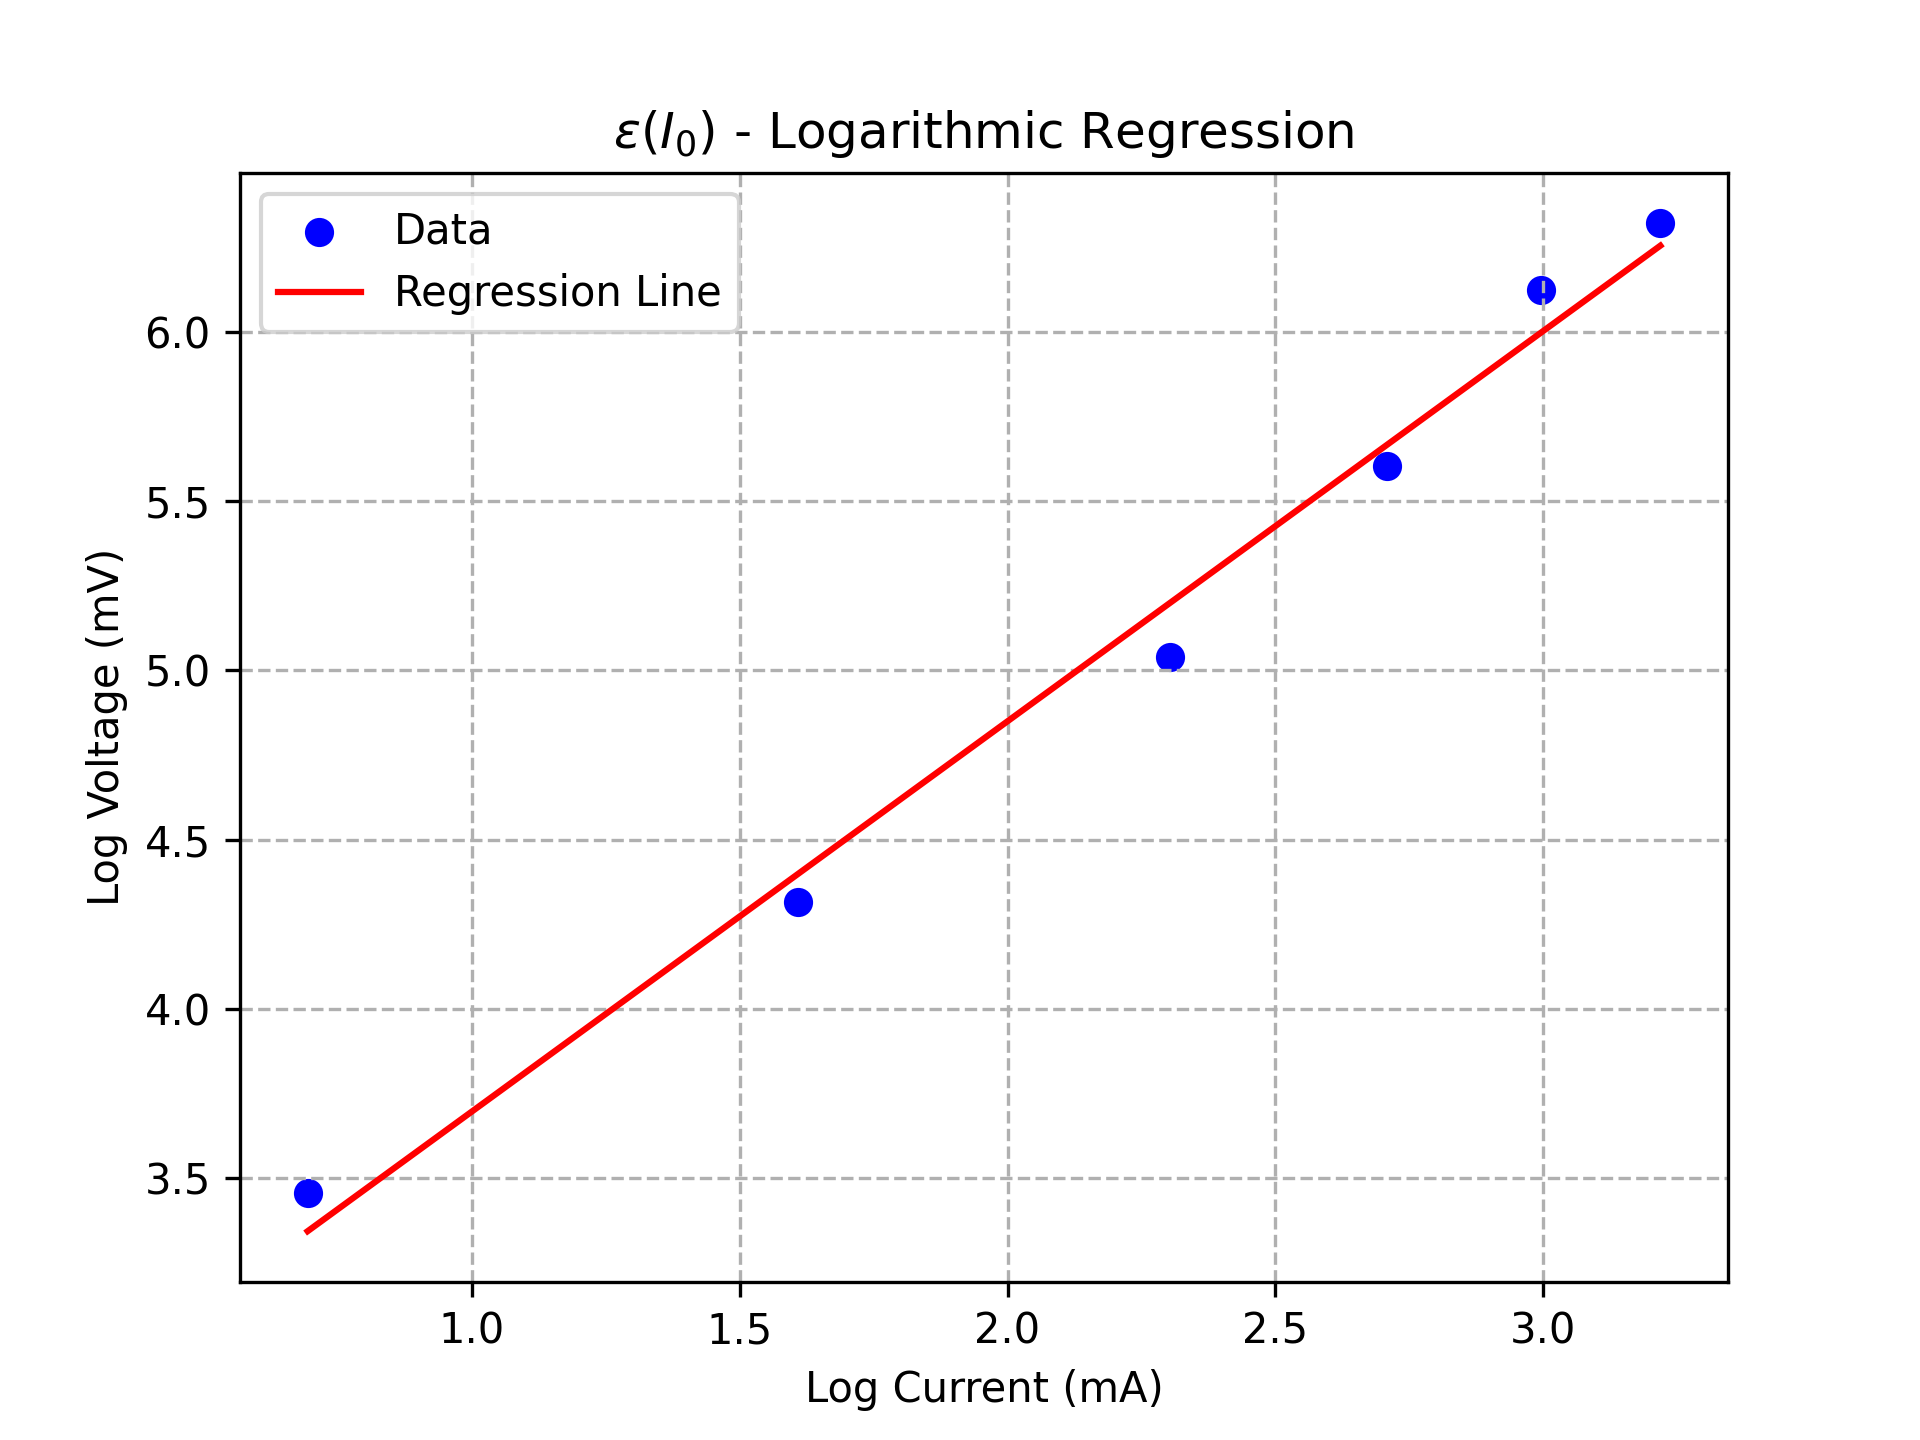
\includegraphics[width=0.9\linewidth]{output_plots/epsilonI_0.png}
    \caption{Induced EMF as a function of Current.}
    \label{fig:epsilon_current}
\end{figure}

\subsection{Induced EMF as a Function of Coil Turns}
Table~\ref{tab:emf_turns} shows the induced EMF for varying numbers of turns in the secondary coil.

\begin{table}[H]
    \centering
    \caption{Induced EMF as a Function of Coil Turns (25 mA, 41 mm diameter)}
    \begin{tabular}{cc}
        \hline
        Turns (n) & EMF (mV) \\ \hline
        300 & 556 \\
        200 & 350 \\ 
        100 & 150 \\\hline
    \end{tabular}
    \label{tab:emf_turns}
\end{table}

The graph for EMF as a function of coil turns is shown in Fig.~\ref{fig:epsilon_turns}.

\begin{figure}[H]
    \centering
    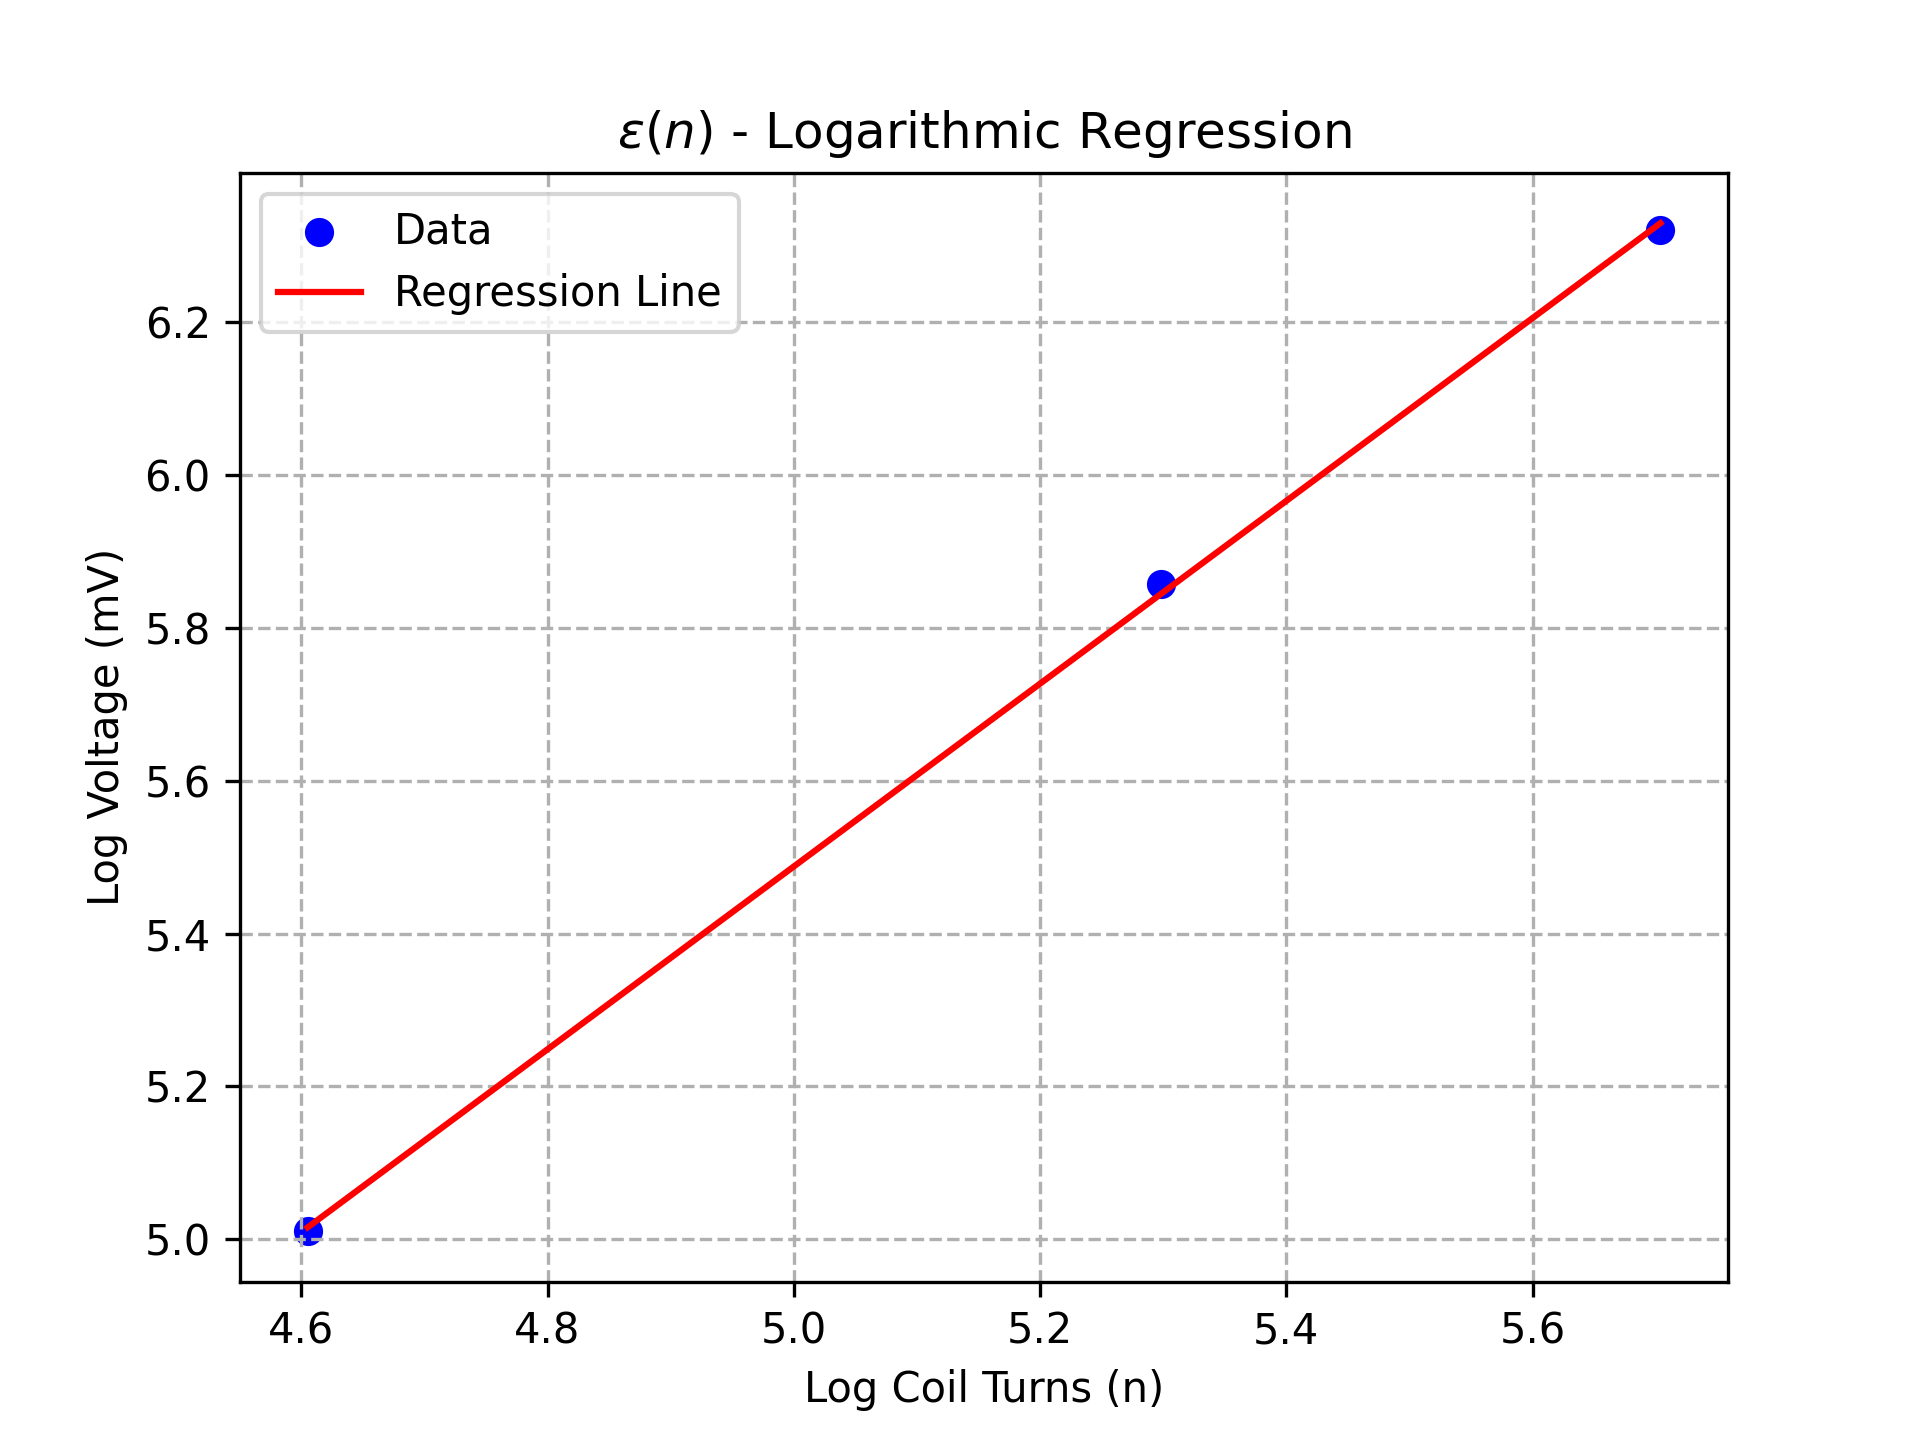
\includegraphics[width=0.9\linewidth]{output_plots/epsilonN.png}
    \caption{Induced EMF as a function of Coil Turns.}
    \label{fig:epsilon_turns}
\end{figure}

\subsection{Induced EMF as a Function of Coil Diameter}
The induced EMF for coils with different diameters is presented in Table~\ref{tab:emf_diameter}.

\begin{table}[H]
    \centering
    \caption{Induced EMF as a Function of Coil Diameter (25 mA, 300 turns)}
    \begin{tabular}{cc}
        \hline
        Diameter (mm) & EMF (mV) \\ \hline
        41 & 556 \\
        33 & 338 \\
        26 & 183 \\ \hline
    \end{tabular}
    \label{tab:emf_diameter}
\end{table}

The graph for EMF as a function of coil diameter is shown in Fig.~\ref{fig:epsilon_diameter}.

\begin{figure}[H]
    \centering
    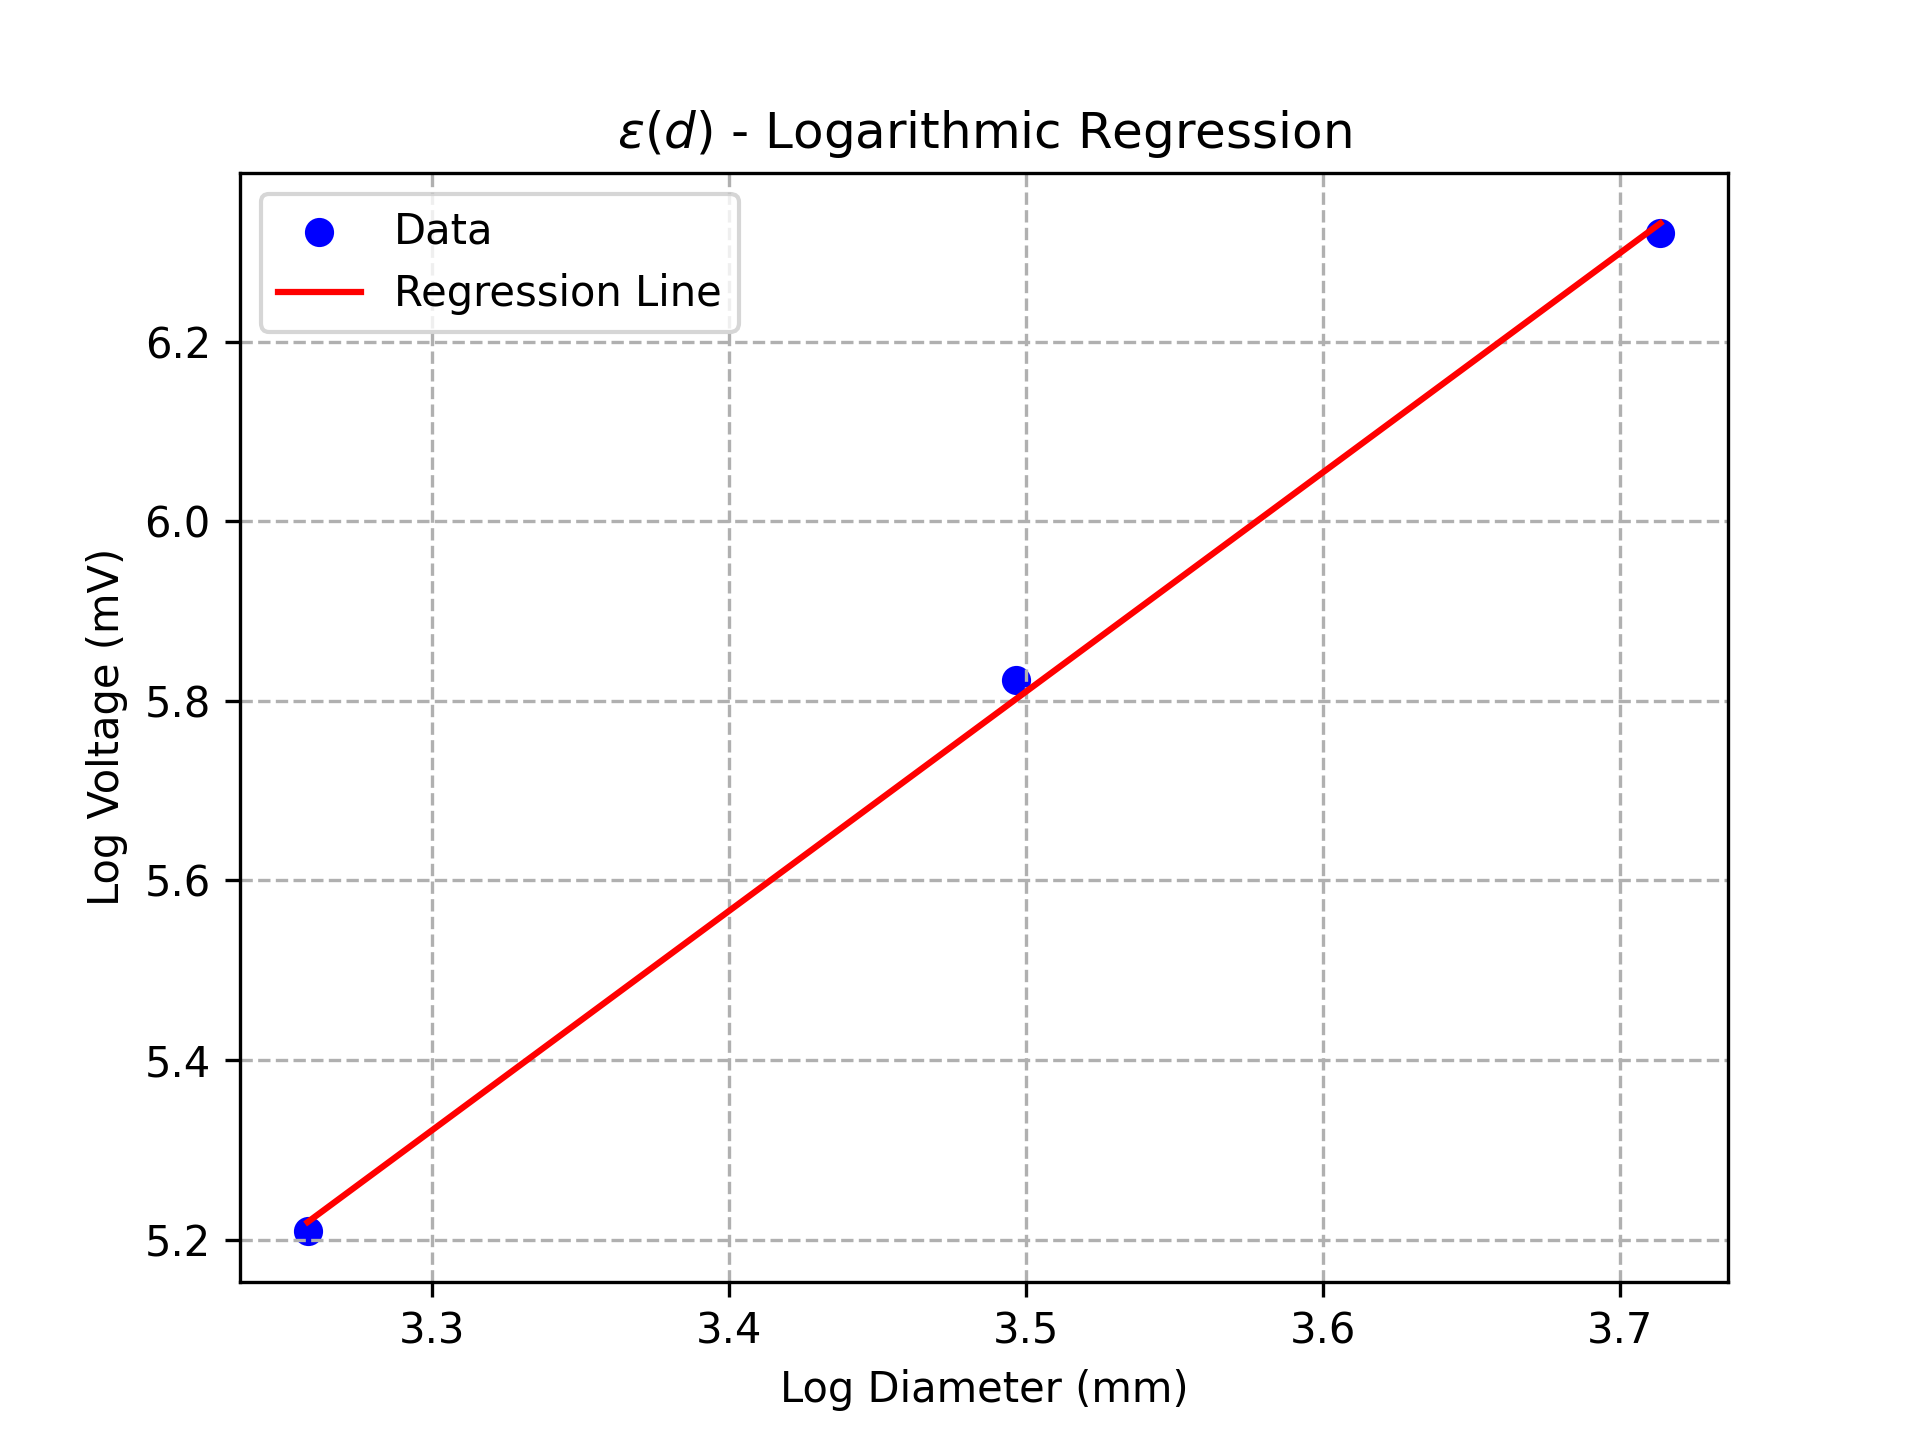
\includegraphics[width=0.9\linewidth]{output_plots/epsilonD.png}
    \caption{Induced EMF as a function of Coil Diameter.}
    \label{fig:epsilon_diameter}
\end{figure}

\section{Discussion}
The results confirm the theoretical relationships governing electromagnetic induction. In Part I, we observed that the induced EMF increased as the current in the primary coil increased, consistent with the proportional relationship predicted by Faraday’s Law. The log-log plot of \(\varepsilon\) vs. \(I\) (not shown here) yielded a linear relationship, confirming that \(\varepsilon \propto I\).

In Part II, the induced EMF increased with the number of turns in the secondary coil, as expected from the equation:
\begin{equation}
    \varepsilon \propto n_2
\end{equation}
Finally, in Part III, increasing the diameter of the secondary coil resulted in higher induced EMF, as larger coils enclose more magnetic flux.

\section{Conclusion}
This experiment successfully demonstrated the principles of electromagnetic induction using coils. The induced EMF was found to be directly proportional to the current in the primary coil, the number of turns in the secondary coil, and the diameter of the coil. The results align well with theoretical predictions, confirming the validity of Faraday's Law in practical scenarios.

\section{Additional Resources}
For further analysis, you can find supplementary resources in the QR code links below.

\begin{figure}[H]
    \centering
    \qrcode{https://drive.google.com/folder/view?usp=sharing}
    \caption{Link to Supplementary Data}
\end{figure}

\end{document}
